\documentclass[a4paper,12pt]{article}
\usepackage[utf8x]{inputenc} % Codifica UTF-8
\usepackage[italian]{babel} % Lingua italiana
\usepackage[T1]{fontenc}
\usepackage{amsmath} % Simboli matematici
\usepackage{siunitx} % Unità di misura
\usepackage{listings} % Inserimento codice
\usepackage{graphicx} % Inserimento immagini
\usepackage{caption} % Didattiche delle figure
\usepackage{hyperref} % Riferimenti ipertestuali
\usepackage{xcolor}
\usepackage{float}
\definecolor{grey}{rgb}{0.5, 0.5, 0.5}
% Configurazione per il codice Python
\definecolor{mybackgroundcolor}{rgb}{0.95, 0.95, 0.95}
\definecolor{mykeywordcolor}{rgb}{0.9, 0.0, 0.0}
\lstset{ 
    backgroundcolor=\color{mybackgroundcolor}, % Colore di sfondo
    basicstyle=\footnotesize\ttfamily, % Dimensione del font e tipo
    keywordstyle=\color{mykeywordcolor}, % Colore delle parole chiave
    commentstyle=\color{gray}, % Colore dei commenti
    stringstyle=\color{red}, % Colore delle stringhe
    frame=single, % Bordo attorno al listato
    breaklines=true, % Ritorno a capo automatico
    numbers=none, %non numera i codici
    captionpos=b % Posizione della didascalia
}
\usepackage{amsmath}










\title{Analisi Statistica dei Dati Sperimentali}
\author{Laboratorio di Fisica}
\date{}

\begin{document}

\maketitle

\section{Introduzione}
In questo capitolo esploreremo l'analisi statistica dei dati sperimentali utilizzando Python. Gli argomenti trattati includeranno la gestione delle misure come variabili casuali, la funzione di distribuzione normale, l'uso di matplotlib per la visualizzazione dei dati e la regressione lineare. Eseguiremo anche un esempio completo per il calcolo dell'accelerazione di gravità.

\section{Misure come Variabili Casuali}
Le misure sperimentali sono trattate come variabili casuali, il che implica che i valori misurati sono soggetti a variazioni casuali dovute a errori di misurazione e condizioni sperimentali. Tutto questo, nell'ipotesi che la sensibilità degli strumenti non copra le fluttuazioni casuali. Se misuro la lunghezza di un tavolo 40 volte, otterrò sempre lo stesso valore, se uso un metro da falegname. In tal caso la statistica è inutile perché i dati non mostrano alcuna variabilità. Se però misuro il tempo di caduta di una pallina che viene lasciata cadere da una persona e lo faccio con un cronometro manule, otterrò diversi valori e in tal caso ha senso fare un'analisi statistica. Nelle pagine che seguono, supporremo di fare misure che esibiscono una certa variabilità. Un esempio è la misura delle altezze di una popolazione di persone (ad esempio uomini della stessa età). Sappiamo che otterremo una certa variazione ma in tal caso la variabilità non è legata alla persona che esegue le misure ma alla grandezza fisica stessa: le altezze non sono tutte uguali! La statistica, però, non fà distinzione tra questi due casi e si occupa di capire due cose: 1) Qual è il valore medio della grandezza; 2) Come varia questa proprietà. 100 uomini di un gruppo A, potrebbero avere un'altezza media di 1,75 m e cosi anche 100 uomini di un gruppo B ma con una grande variabilità (ad esempio 5 uomini sotto i 160 cm, 5 uominitra 160 cm e 165 cm, 5 uomini tra 165 cm e 170 cm e così via. Nel gruppo A invece, magari i 3/4 degli uomini hanno un'altezza molto vicina alla media. In fisica, lo ''sparpagliamento'' dei risultati, viene identificato con quello che abbiamo chiamato errore assoluto o incertezza in quanto ci dà una misura di quanto è precisa la nostra misurazione. Se faccio oscillare un pendolo e misuro i periodi (la durata di un'oscillazione) e il cronometro ha una sensibilità di 0,01 s, ma in media i miei valori si discostano dal valore medio per 0,5 secondi, allora prenderò questa come misura di incertezza.











\section{Uso di Matplotlib per la Visualizzazione dei Dati}

Matplotlib è una libreria potente per la creazione di grafici in Python. Di seguito è riportato un esempio di come realizzare un grafico delle misure sperimentali con barre di errore.

\subsection{Esempio di Grafico}

Consideriamo  i  dati nella tabella \ref{tab:datia}:

\begin{table}[!h]
    \centering
    \begin{tabular}{|c|c|}
        \hline
        \textbf{Variabile indipendente (\(x\))} & \textbf{Variabile dipendente (\(y\))} \\
        \hline
        0 & 0.5 \\
        1.11 & 3.1 \\
        2.22 & 5.2 \\
        3.33 & 8.3 \\
        4.44 & 11.1 \\
        5.55 & 13.9 \\
        6.66 & 16.5 \\
        7.77 & 19.4 \\
        8.88 & 22.1 \\
        10 & 25.3 \\
        \hline
    \end{tabular}
    \caption{Dati di \(x\) e \(y\) utilizzati nel grafico}
    \label{tab:datia}
\end{table}

Il codice Python per realizzare il grafico è:

\begin{lstlisting}[caption={Grafico delle misure sperimentali con barre di errore}]
import matplotlib.pyplot as plt
import numpy as np

# Dati di esempio assegnati esplicitamente
x = np.array([0, 1.11, 2.22, 3.33, 4.44, 5.55, 6.66, 7.77, 8.88, 10])
y = np.array([0.5, 3.1, 5.2, 8.3, 11.1, 13.9, 16.5, 19.4, 22.1, 25.3])
yerr = np.array([0.6, 0.4, 0.5, 0.3, 0.7, 0.2, 0.4, 0.6, 0.5, 0.3])  # Assicurarsi che yerr sia positivo

# Creazione della figura e dell'asse
fig, ax = plt.subplots()

# 

ax.errorbar(x, y, yerr=yerr, fmt='o', ecolor='red', capsize=5, label='Misure sperimentali')

# Aggiunta di etichette agli assi
ax.set_xlabel('Variabile indipendente')
ax.set_ylabel('Variabile dipendente')

# Aggiunta di un titolo
ax.set_title('Grafico delle Misure Sperimentali con Barre di Errore')

# Aggiunta di una legenda
ax.legend()

# Aggiunta di una griglia
ax.grid(True)
# Stampa il grafico
plt.savefig('grafico-misure.png')
# Mostra il grafico
plt.show()
#se vuoi scaricare il file da google colab decommenta le righe:
#from google.colab import files
#files.download('grafico-misure.png')

\end{lstlisting}

\section{Spiegazione del Codice per un Grafico Sperimentale}

\subsection{Importazione delle librerie}
\begin{lstlisting}[language=Python, caption=Importazione delle librerie]
import matplotlib.pyplot as plt
import numpy as np
\end{lstlisting}
Il codice sopra importa le librerie necessarie per la creazione del grafico. La libreria \texttt{matplotlib.pyplot} fornisce strumenti per la creazione di grafici e visualizzazioni, mentre \texttt{numpy} è fondamentale per operazioni numeriche e manipolazione di array.

\subsection{Dati di esempio}
\begin{lstlisting}[language=Python, caption=Dati di esempio]
x = np.array([0, 1.11, 2.22, 3.33, 4.44, 5.55, 6.66, 7.77, 8.88, 10])
y = np.array([0.5, 3.1, 5.2, 8.3, 11.1, 13.9, 16.5, 19.4, 22.1, 25.3])
yerr = np.array([0.6, 0.4, 0.5, 0.3, 0.7, 0.2, 0.4, 0.6, 0.5, 0.3])
\end{lstlisting}
Questi array contengono i dati di esempio per il grafico. L'array \texttt{x} rappresenta i valori della variabile indipendente, mentre \texttt{y} rappresenta i valori della variabile dipendente. \texttt{yerr} contiene gli errori associati ai valori di \texttt{y}.

\subsection{Creazione della figura e dell'asse}
\begin{lstlisting}[language=Python, caption=Creazione della figura e dell'asse]
fig, ax = plt.subplots()
\end{lstlisting}
Questa riga di codice crea una nuova figura e un asse (grafico). La variabile \texttt{fig} rappresenta la figura, mentre \texttt{ax} è l'asse su cui viene tracciato il grafico.

\subsection{Creazione del grafico con barre di errore}
\begin{lstlisting}[language=Python, caption=Creazione del grafico con barre di errore]
ax.errorbar(x, y, yerr=yerr, fmt='o', ecolor='red', capsize=5, label='Misure sperimentali')
\end{lstlisting}
Questo comando crea un grafico a dispersione con barre di errore. I parametri specificati sono:
\begin{itemize}
    \item \texttt{x}: Array dei valori dell'asse x.
    \item \texttt{y}: Array dei valori dell'asse y.
    \item \texttt{yerr}: Array degli errori associati ai valori di \texttt{y}.
    \item \texttt{fmt='o'}: Specifica che i punti dati devono essere rappresentati come cerchi.
    \item \texttt{ecolor='red'}: Colore delle barre di errore (rosso in questo caso).
    \item \texttt{capsize=5}: Dimensione delle estremità delle barre di errore.
    \item \texttt{label='Misure sperimentali'}: Etichetta da utilizzare nella legenda per il grafico a dispersione.
\end{itemize}

\subsection{Aggiunta di etichette agli assi}
\begin{lstlisting}[language=Python, caption=Aggiunta di etichette agli assi]
ax.set_xlabel('Variabile indipendente')
ax.set_ylabel('Variabile dipendente')
\end{lstlisting}
Queste righe di codice aggiungono etichette agli assi del grafico. \texttt{ax.set\_xlabel} aggiunge un'etichetta all'asse delle ascisse (x), mentre \texttt{ax.set\_ylabel} aggiunge un'etichetta all'asse delle ordinate (y).

\subsection{Aggiunta di un titolo}
\begin{lstlisting}[language=Python, caption=Aggiunta di un titolo]
ax.set_title('Grafico delle Misure Sperimentali con Barre di Errore')
\end{lstlisting}
Questa riga di codice aggiunge un titolo al grafico.

\subsection{Aggiunta di una legenda}
\begin{lstlisting}[language=Python, caption=Aggiunta di una legenda]
ax.legend()
\end{lstlisting}
Il comando \texttt{ax.legend()} aggiunge una legenda al grafico, mostrando le etichette dei dati.

\subsection{Aggiunta di una griglia}
\begin{lstlisting}[language=Python, caption=Aggiunta di una griglia]
ax.grid(True)
\end{lstlisting}
Questa riga di codice aggiunge una griglia al grafico, facilitando la lettura dei valori.

\subsection{Visualizzazione del grafico}
\begin{lstlisting}[language=Python, caption=Visualizzazione del grafico]
plt.show()
\end{lstlisting}
Infine, \texttt{plt.show()} visualizza il grafico creato. Senza questo comando, il grafico non verrà visualizzato.

\section{Istogrammi a Bins}
Un istogramma è una rappresentazione grafica della distribuzione di un insieme di dati. Esso suddivide l'intervallo dei dati in una serie di intervalli chiamati bins (o classi) e conta il numero di dati che rientrano in ciascun bin. L'altezza di un rettangolo è pari alla frequenza, ossia è pari al rapporto tra le misure  comprese tra i due estremi della base del rettangolo  e il totale delle misure.  In figura \ref{fig:istogrammagenerico} vediamo un tipico istogramma.

\begin{figure}[h!]
    \centering
    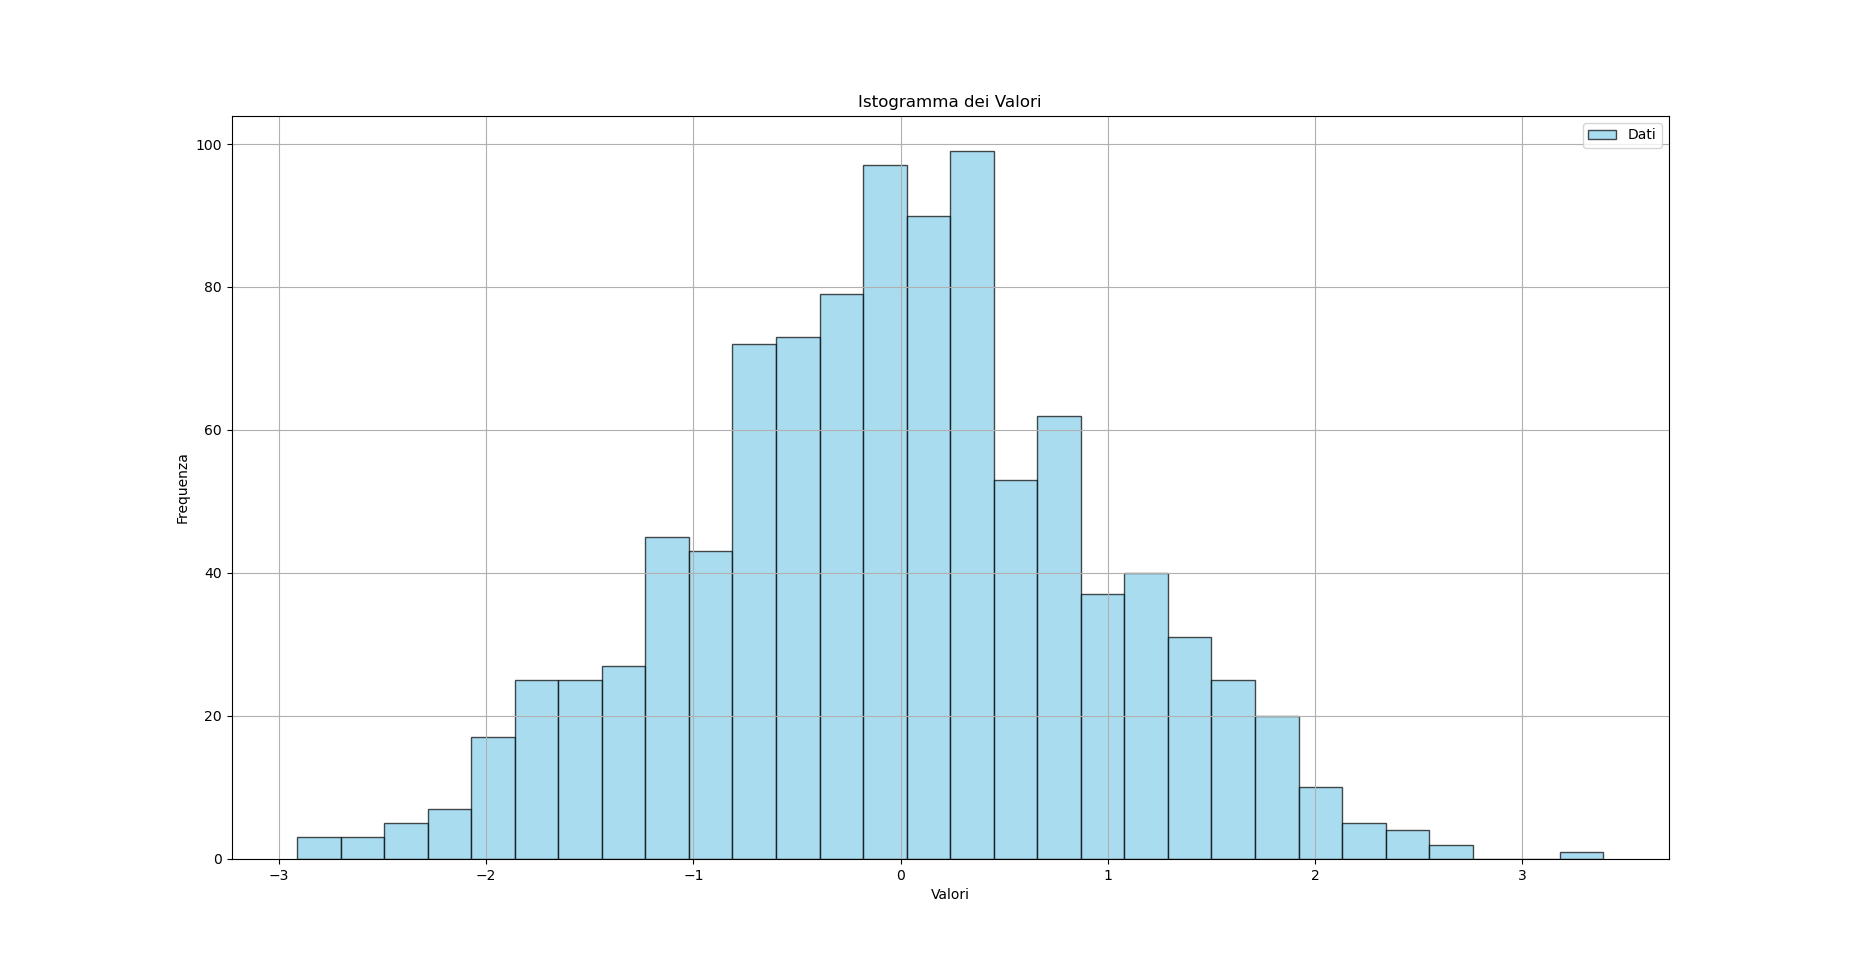
\includegraphics[width=\linewidth]{istogrammagenerico.png}
    \caption{Istogramma dei Valori}
    \label{fig:istogrammagenerico}
\end{figure}


 
L'ampiezza dei bins può influenzare significativamente l'aspetto dell'istogramma. Bins più stretti possono mostrare più dettagli, ma possono anche evidenziare il rumore nei dati, mentre bins più larghi forniscono una visione più smussata della distribuzione. La scelta del numero di suddivisioni dipende dal numero di dati: se si hanno molti dati si possono prendere più bins. Si consiglia di fare dei tentativi. Se l'istogramma rappresenta una distribuzione gaussiana  (detta anche ''normale``) il suo aspetto deve ricordare quello di una campana. Ne parleremo nei prossimi paragrafi in cui useremo il linguaggio Python per disegnare un'istogramma, dunque non ci dovremo preoccupare di disegnarlo a mano ma è importante conoscere il significato di questo tipo di diagramma. Questo linguaggio offre maggiori personalizzazioni dei semplici grafici realizzati da excel. Il grafico in figura è stato realizzato col codice python:




\begin{lstlisting}[ caption={Script Python per disegnare un'istogramma}]
import matplotlib.pyplot as plt
import numpy as np

# Dati di esempio
data = np.random.randn(1000)

# Creazione della figura e dell'asse
fig, ax = plt.subplots()

# Creazione dell'istogramma
n, bins, patches = ax.hist(data, bins=30, color='skyblue', edgecolor='black', alpha=0.7)

# Aggiunta di etichette agli assi
ax.set_xlabel('Valori')
ax.set_ylabel('Frequenza')

# Aggiunta di un titolo
ax.set_title('Istogramma dei Valori')

# Aggiunta di una legenda
ax.legend(['Dati'])

# Aggiunta di una griglia
ax.grid(True)
plt.savefig('istogramma.png')
#se vuoi scaricare il file da google colab decommenta le righe:
#from google.colab import files
#files.download('istogramma.png')
# Mostra il grafico
plt.show()



\end{lstlisting}

\section{Spiegazione del Codice per creare un'istogramma}
\subsection{Importazione delle Librerie}
Il codice inizia importando le librerie necessarie:
\begin{lstlisting}[language=Python]
import matplotlib.pyplot as plt
import numpy as np
\end{lstlisting}
\texttt{matplotlib.pyplot} è utilizzata per creare grafici, mentre \texttt{numpy} è utilizzata per gestire gli array di dati.

\subsection{Generazione dei Dati}
I dati di esempio sono generati utilizzando la funzione \texttt{randn} di \texttt{numpy}, che crea un array di 1000 numeri casuali con distribuzione normale:
\begin{lstlisting}[language=Python]
data = np.random.randn(1000)
\end{lstlisting}

\subsection{Creazione della Figura e dell'Asse}
Viene creata una figura e un asse per il grafico:
\begin{lstlisting}[language=Python]
fig, ax = plt.subplots()
\end{lstlisting}

\subsection{Creazione dell'Istogramma}
L'istogramma viene creato utilizzando la funzione \texttt{hist}:
\begin{lstlisting}[language=Python]
n, bins, patches = ax.hist(data, bins=30, color='skyblue', edgecolor='black', alpha=0.7)
\end{lstlisting}
\texttt{bins=30} specifica il numero di intervalli, \texttt{color='skyblue'} imposta il colore delle barre, \texttt{edgecolor='black'} imposta il colore dei bordi delle barre, e \texttt{alpha=0.7} imposta la trasparenza delle barre.

\subsection{Aggiunta di Etichette e Titolo}
Vengono aggiunte etichette agli assi e un titolo al grafico:
\begin{lstlisting}[language=Python]
ax.set_xlabel('Valori')
ax.set_ylabel('Frequenza')
ax.set_title('Istogramma dei Valori')
\end{lstlisting}

\subsection{Aggiunta di una Legenda e di una Griglia}
Infine, vengono aggiunte una legenda e una griglia al grafico:
\begin{lstlisting}[language=Python]
ax.legend(['Dati'])
ax.grid(True)
\end{lstlisting}

\subsection{Visualizzazione del Grafico}
Il grafico viene visualizzato con il comando:
\begin{lstlisting}[language=Python]
plt.show()
\end{lstlisting}

\section{Esempio di istogramma sperimentale}

\subsection{Introduzione}
In questo esempio, verranno presentati i dati di un esperimento di misura fisica, la fisica sottostante e il processo per creare un istogramma che rappresenti questi dati utilizzando il linguaggio di programmazione Python con la libreria Matplotlib.

\subsection{Descrizione dell'esperimento}
L'esperimento consiste nel misurare la lunghezza di un campione di barre metalliche. Le misure sono state effettuate utilizzando un calibro digitale con una precisione di 0.1 mm. Di seguito sono riportati i dati sperimentali ottenuti (in cm):

\[
\begin{array}{cccccc}
45.1 & 47.2 & 49.3 & 50.5 & 52.6 & 54.7 \\
48.3 & 46.9 & 51.2 & 53.8 & 50.0 & 49.9 \\
48.7 & 51.5 & 52.1 & 47.6 & 46.3 & 50.9 \\
51.8 & 48.0 & 49.5 & 50.3 & 47.0 & 46.5 \\
52.4 & 48.8 & 49.2 & 51.3 & 47.8 & 50.7 \\
\end{array}
\]
Nel contesto della statistica, useremo solo programmi software e ci disinteresseremo dei problemi relativi alle cifre significative durante i calcoli, mentre queste saranno importanti nel momento in cui scriveremo il risultato delle misure.
\subsection{Fisica dell'esperimento}
La misura della lunghezza delle barre metalliche è un esperimento comune in fisica per studiare le proprietà dei materiali. La lunghezza può variare a causa di fattori come:
\begin{itemize}
    \item Differenze nel processo di produzione.
    \item Espansione termica a diverse temperature.
    \item Errori sistematici e casuali durante la misurazione.
\end{itemize}
L'istogramma delle misure permette di visualizzare la distribuzione delle lunghezze e di identificare eventuali deviazioni significative dalla media.

\subsection{Creazione dell'istogramma con Python}
Per creare l'istogramma, utilizziamo il seguente codice Python:

\begin{lstlisting}[language=Python, caption=Codice Python per creare l'istogramma]
import matplotlib.pyplot as plt

# Dati sperimentali
dati_sperimentali = [45.1, 47.2, 49.3, 50.5, 52.6, 54.7, 48.3, 46.9, 51.2, 53.8, 
                     50.0, 49.9, 48.7, 51.5, 52.1, 47.6, 46.3, 50.9, 51.8, 48.0, 
                     49.5, 50.3, 47.0, 46.5, 52.4, 48.8, 49.2, 51.3, 47.8, 50.7]

# Crea l'istogramma
plt.figure(figsize=(10, 6))
plt.hist(dati_sperimentali, bins=8, edgecolor='black', alpha=0.7)

# Aggiungi titolo e etichette
plt.title('Istogramma dei dati sperimentali')
plt.xlabel('Misura (cm)')
plt.ylabel('Frequenza')

# Mostra l'istogramma
plt.savefig('istogramma2.png')  # Salva l'immagine come istogramma2.png
plt.show()
\end{lstlisting}

\subsubsection{Spiegazione del codice}
Il codice Python utilizzato per creare l'istogramma è spiegato di seguito:

\paragraph{Importazione delle librerie}
\begin{lstlisting}[language=Python, caption=Importazione delle librerie]
import matplotlib.pyplot as plt
\end{lstlisting}
Questo codice importa la libreria Matplotlib, necessaria per la creazione di grafici.

\paragraph{Definizione dei dati}
\begin{lstlisting}[language=Python, caption=Definizione dei dati]
dati_sperimentali = [45.1, 47.2, 49.3, 50.5, 52.6, 54.7, 48.3, 46.9, 51.2, 53.8, 
                     50.0, 49.9, 48.7, 51.5, 52.1, 47.6, 46.3, 50.9, 51.8, 48.0, 
                     49.5, 50.3, 47.0, 46.5, 52.4, 48.8, 49.2, 51.3, 47.8, 50.7]
\end{lstlisting}
Definisce un array contenente i dati delle misurazioni fisiche.

\paragraph{Creazione dell'istogramma}
\begin{lstlisting}[language=Python, caption=Creazione dell'istogramma]
plt.figure(figsize=(10, 6))
plt.hist(dati_sperimentali, bins=8, edgecolor='black', alpha=0.7)
\end{lstlisting}
Imposta la dimensione della figura e crea un istogramma con 8 bin, bordi neri per i bin e trasparenza del 70\%.

\paragraph{Aggiunta di titolo e etichette}
\begin{lstlisting}[language=Python, caption=Aggiunta di titolo e etichette]
plt.title('Istogramma dei dati sperimentali')
plt.xlabel('Misura (cm)')
plt.ylabel('Frequenza')
\end{lstlisting}
Aggiunge il titolo e le etichette agli assi del grafico.

\paragraph{Visualizzazione e salvataggio dell'istogramma}
\begin{lstlisting}[language=Python, caption=Visualizzazione e salvataggio dell'istogramma]
plt.savefig('istogramma2.png')  # Salva l'immagine come istogramma2.png
plt.show()
\end{lstlisting}
Visualizza l'istogramma generato e lo salva come `istogramma2.png`.

\subsection{Risultati}
L'istogramma risultante mostra la distribuzione delle lunghezze delle barre metalliche. L'analisi visiva dell'istogramma permette di identificare la variabilità delle misurazioni e la presenza di eventuali outlier.

\begin{figure}[H]
    \centering
    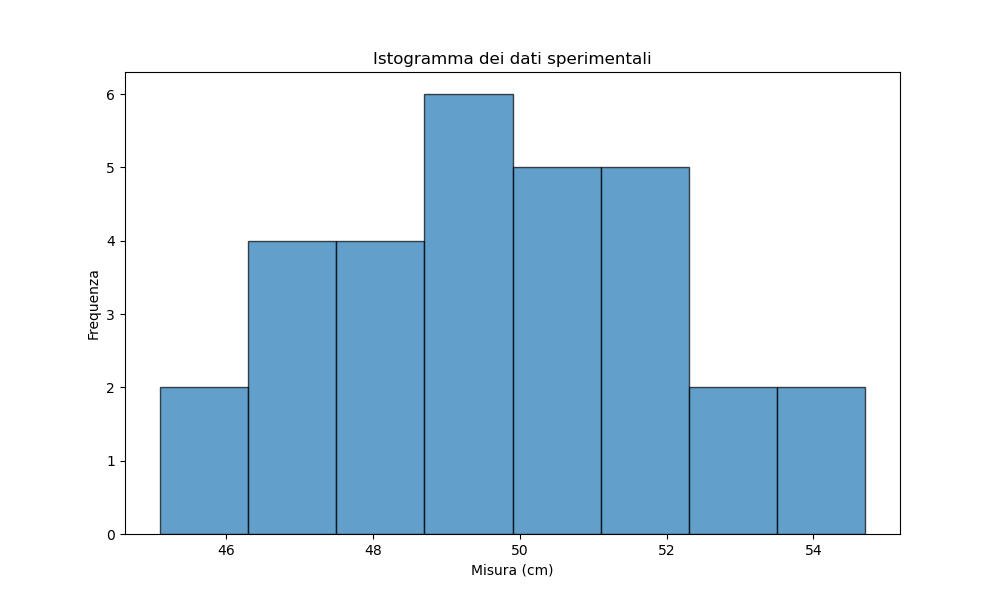
\includegraphics[width=0.8\textwidth]{istogramma2.png}
    \caption{Istogramma dei dati sperimentali}
    \label{fig:istogramma}
\end{figure}

\section{Distribuzione di Probabilità}
In questa e nelle prossime sezioni, parleremo di probabilità. Quando misuriamo una grandezza casuale, vediamo che alcuni valori si ripetono più frequentemente di altri, ossia abbiamo una \textit{distribuzione} di valori. La statistica ci permette di estrarre da questa distribuzione, informazioni sulla grandezza. Si suppone che ogni grandezza abbia un valore ''vero`` e che solo effetti casuali discostino il risultato da quest'ultimo. La distribuzione dei valori viene misurata non tanto dalla semidispersione massima (una stima troppo grande) ma dalla deviazione standard (un concetto statistico). Ripetendo le misure molte volte, costruendo un   \textbf{istogramma delle frequenze}, otteniamo che questo istogramma diventa sempre  più liscio e  si avvicina ad una curva a forma di campana. In fisica, questa curva si presenta quando ripetiamo molte volte una misura casuale. In quel caso, la grandezza non ha sempre lo stesso valore ma ha, appunto, una \textit{distribuzione}. Se facciamo oscillare un pendolo, e misuriamo la durata $t$ di 20 oscillazioni con un cronometro manuale, non otterremo quasi mai due volte lo stesso valore (a causa di errori umani) ma una serie di valori. La statistica ci consente di prevedere quali saranno i valori più probabili e come questi si distribuiscono, (quanti ad esempio sono molto più grandi o più piccoli della media). Le prossime sezioni ci insegneranno come trarre informazioni utili dalla distribuzione di queste misure. Impareremo che il risultato di una misura è dato dalla media e dall'errore della media, come segue:
\[
x=\left(\overline{x} \pm \sigma_{\overline{x}}\right) \, \text{u.m.}
\]
essendo $\overline{x}$ la media dei valori e $\sigma_{\overline{x}}$ la cosiddetta deviazione standard della media.

\subsection{La Curva di Gauss}

La distribuzione gaussiana è caratterizzata dalla seguente funzione densità di probabilità (pdf):

\begin{equation}
f(x|\mu,\sigma) = \frac{1}{\sigma \sqrt{2\pi}} e^{-\frac{(x-\mu)^2}{2\sigma^2}}
\label{eq:gauss}
\end{equation}

dove:
\begin{itemize}
    \item $\mu$ è la media della distribuzione, che indica il valore centrale attorno al quale i dati sono distribuiti.
    \item $\sigma$ è la deviazione standard, che misura la dispersione dei dati rispetto alla media.
\end{itemize}
Non spaventatevi, non importa il significato di tutti i i simboli, non useremo direttamente la formula. A voi basta sapere che questa è una relazione tra quello che c'è a sinistra dell'uguale e quello che c'è a destra.  
La curva di Gauss ha una forma a campana, simmetrica rispetto alla media $\mu$. La maggior parte dei dati (circa il 68\%) si trova entro un intervallo di una deviazione standard dalla media ($\mu \pm \sigma$), mentre il 95\% dei dati si trova entro due deviazioni standard ($\mu \pm 2\sigma$). Questo comportamento rende la distribuzione gaussiana particolarmente utile per descrivere fenomeni naturali dove le variazioni sono dovute a molti fattori piccoli e indipendenti. In figura \ref{fig:curva_gaussiana} vediamo il tipico aspetto di una gaussiana.

\begin{figure}[h!]
    \centering
     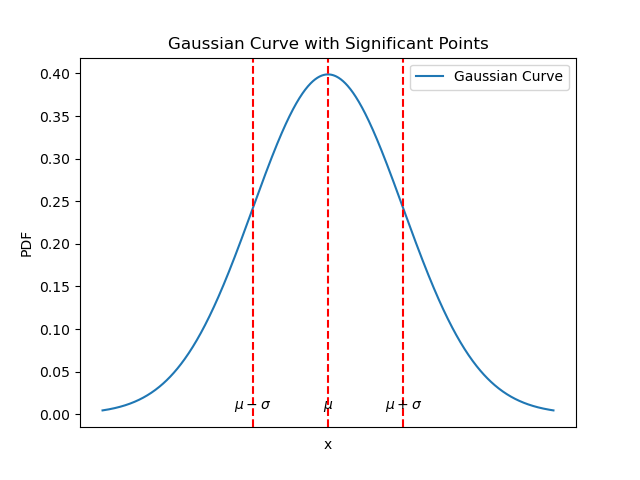
\includegraphics[scale=0.7]{curva_gaussiana.png} 
    \caption{Curva Gaussiana con Evidenziati \(\overline{x}\), \(\overline{x} - \sigma\), e \(\overline{x} + \sigma\)}
    \label{fig:curva_gaussiana}
\end{figure}









\section{Stima di Media e Deviazione Standard}
Data una serie di $n$ misurazioni sperimentali $\{x_1, x_2, \ldots, x_n\}$, possiamo stimare i parametri della distribuzione gaussiana, cioè la media $\mu$ e la deviazione standard $\sigma$, utilizzando le seguenti formule:

\subsection{Calcolo della Media}
La media campionaria $\hat{\mu}$ è data dalla somma di tutte le osservazioni divisa per il numero totale di osservazioni:

\begin{equation}
\hat{\mu} = \frac{1}{n} \sum_{i=1}^{n} x_i
\end{equation}

\subsection{Calcolo della Deviazione Standard}
La deviazione standard campionaria $\hat{\sigma}$ è data dalla radice quadrata della somma dei quadrati delle differenze tra ciascuna osservazione e la media campionaria, divisa per il numero di osservazioni meno uno:

\begin{equation}
\hat{\sigma} = \sqrt{\frac{1}{n-1} \sum_{i=1}^{n} (x_i - \hat{\mu})^2}
\end{equation}

\subsection{Calcolo della Deviazione Standard della Media}
La deviazione standard della media, nota anche come errore standard della media, è calcolata come:

\begin{equation}
\sigma_{\overline{x}} = \frac{\hat{\sigma}}{\sqrt{n}}
\end{equation}

Dove $\hat{\sigma}$ è la deviazione standard campionaria e $n$ è il numero di osservazioni. La deviazione standard della media rappresenta quanto la media campionaria è attesa essere distante dalla media vera della popolazione. Per una stima più precisa, questa deviazione standard della media viene approssimata a una cifra significativa.




\section{Esempio: istogramma e distribuzione}
Per illustrare questi concetti, consideriamo un esempio pratico in Python. Abbiamo misurato le altezze di 100 persone (in cm) e calcoleremo la media, la deviazione standard e la deviazione standard della media di queste misure. Successivamente, creeremo un istogramma delle altezze e lo sovrapporremo con la curva gaussiana corrispondente.

\begin{lstlisting}[caption={Script Python per calcolare e visualizzare le altezze}]
import numpy as np
import matplotlib.pyplot as plt
from scipy.stats import norm

# Altezze di 100 persone (in cm)
heights = [170, 165, 180, 175, 160, 155, 178, 172, 168, 169, 
           174, 167, 166, 171, 173, 177, 182, 181, 176, 179, 
           164, 163, 162, 161, 159, 158, 157, 156, 154, 153, 
           152, 151, 150, 149, 148, 147, 146, 145, 144, 143,
           150, 155, 160, 165, 170, 175, 180, 185, 190, 195,
           172, 177, 182, 187, 192, 197, 162, 167, 172, 177,
           180, 175, 170, 165, 160, 155, 150, 145, 140, 135,
           142, 147, 152, 157, 162, 167, 172, 177, 182, 187,
           165, 170, 175, 180, 185, 190, 195, 200, 205, 210]

# Stima di media, deviazione standard e deviazione standard della media
mu = np.mean(heights)
sigma = np.std(heights, ddof=1)
sigma_x_mean = sigma / np.sqrt(len(heights))

# Arrotonda la deviazione standard della media e la media alle unità
sigma_x_mean_rounded = round(sigma_x_mean)
mu_rounded = round(mu)

print(f"Media delle altezze: {mu_rounded} cm")
print(f"Deviazione standard delle altezze: {sigma:.2f} cm")
print(f"Deviazione standard della media: {sigma_x_mean_rounded} cm")

# Creazione dell'istogramma
count, bins, ignored = plt.hist(heights, bins=6, density=True, alpha=0.6, color='g', edgecolor='black')

# Sovrapposizione della curva gaussiana
xmin, xmax = plt.xlim()
x = np.linspace(xmin, xmax, 100)
p = norm.pdf(x, mu, sigma)
plt.plot(x, p, 'k', linewidth=2)
title = "Istogramma delle Altezze e Curva Gaussiana"
plt.title(title)

# Visualizzazione di media e deviazione standard
plt.axvline(mu, color='r', linestyle='dashed', linewidth=1)
plt.text(mu + mu/10, max(p), f'Media: {mu_rounded} cm', color='r')
plt.axvline(mu + sigma, color='b', linestyle='dashed', linewidth=1)
plt.axvline(mu - sigma, color='b', linestyle='dashed', linewidth=1)
plt.text(mu + sigma + mu/10, max(p)/2, f'Sigma: {sigma:.2f} cm', color='b')
plt.text(mu - sigma - mu/10, max(p)/2, f'Sigma: {sigma:.2f} cm', color='b')

# Impostazione dei valori sui bins come etichette sull'asse x
bin_labels = [f"{int(bins[i])}" for i in range(len(bins))]
plt.xticks(bins, labels=bin_labels, rotation=45)

# Migliora la disposizione dei sottotitoli e delle etichette
plt.tight_layout()

plt.savefig('istogramma.png')
#se vuoi scaricare il file da google colab decommenta le righe:
#from google.colab import files
#files.download('istogramma.png')
plt.show()

# Risultato finale, arrotondato a due cifre significative
print(f"Altezza = ({mu_rounded} ± {sigma_x_mean_rounded}) cm")
\end{lstlisting}


Ecco l'output:
\begin{verbatim}
Media delle altezze: 167.83333333333334 cm
Deviazione standard delle altezze: 15.80 cm
Deviazione standard della media: 1.67 cm
Altezza = (168 ± 2) cm
\end{verbatim}



\section{Spiegazione del Codice per mostrare un istogramma e una gaussiana}

\subsection{Importazione dei Moduli}
\begin{lstlisting}
import matplotlib.pyplot as plt
from scipy.stats import norm
import numpy as np
\end{lstlisting}
Si importano i moduli necessari: \texttt{matplotlib.pyplot} per la creazione dei grafici, \texttt{scipy.stats.norm} per la distribuzione normale e \texttt{numpy} per le operazioni numeriche.

\subsection{Definizione dei Dati}
\begin{lstlisting}
heights = [170, 165, 180, ... , 210]
\end{lstlisting}
Viene creata una lista di altezze di 100 persone in centimetri.

\subsection{Calcolo delle Statistiche}
\begin{lstlisting}
mu = np.mean(heights)
sigma = np.std(heights, ddof=1)
sigma_x_mean = sigma / np.sqrt(len(heights))
\end{lstlisting}
Si calcolano la media (\texttt{mu}), la deviazione standard (\texttt{sigma}) e la deviazione standard della media (\texttt{sigma\_x\_mean}) delle altezze.

\subsection{Arrotondamenti}
\begin{lstlisting}
sigma_x_mean_rounded = round(sigma_x_mean)
mu_rounded = round(mu)
\end{lstlisting}
La media e la deviazione standard della media vengono arrotondate alle unità.

\subsection{Creazione dell'Istogramma}
\begin{lstlisting}
count, bins, ignored = plt.hist(heights, bins=6, density=True, alpha=0.6, color='g', edgecolor='black')
\end{lstlisting}
Viene creato un istogramma delle altezze con 6 bins, normalizzato e colorato di verde con bordo nero.

\subsection{Sovrapposizione della Curva Gaussiana}
\begin{lstlisting}
xmin, xmax = plt.xlim()
x = np.linspace(xmin, xmax, 100)
p = norm.pdf(x, mu, sigma)
plt.plot(x, p, 'k', linewidth=2)
\end{lstlisting}
Si calcolano i limiti dell'asse x, si genera un array di valori e si calcola la densità di probabilità della distribuzione normale. La curva gaussiana viene sovrapposta all'istogramma in nero.

\subsection{Visualizzazione della Media e della Deviazione Standard}
\begin{lstlisting}
plt.axvline(mu, color='r', linestyle='dashed', linewidth=1)
plt.text(mu + mu/10, max(p), f'Media: {mu_rounded} cm', color='r')
plt.axvline(mu + sigma, color='b', linestyle='dashed', linewidth=1)
plt.axvline(mu - sigma, color='b', linestyle='dashed', linewidth=1)
plt.text(mu + sigma + mu/10, max(p)/2, f'Sigma: {sigma:.2f} cm', color='b')
plt.text(mu - sigma - mu/10, max(p)/2, f'Sigma: {sigma:.2f} cm', color='b')
\end{lstlisting}
Vengono disegnate linee verticali tratteggiate per indicare la media e la deviazione standard, con annotazioni per i rispettivi valori.

\subsection{Impostazione delle Etichette dei Bins}
\begin{lstlisting}
bin_labels = [f"{int(bins[i])}" for i in range(len(bins))]
plt.xticks(bins, labels=bin_labels, rotation=45)
\end{lstlisting}
I valori dei bins vengono impostati come etichette sull'asse x, ruotate di 45 gradi.

\subsection{Miglioramento della Disposizione del Grafico}
\begin{lstlisting}
plt.tight_layout()
\end{lstlisting}
Si ottimizza la disposizione dei sottotitoli e delle etichette per evitare sovrapposizioni.

\subsection{Salvataggio e Visualizzazione del Grafico}
\begin{lstlisting}
plt.savefig('istogramma.png')
plt.show()
\end{lstlisting}
Il grafico viene salvato come immagine \texttt{istogramma.png} e visualizzato a schermo.

\subsection{Risultato Finale}
\begin{lstlisting}
print(f"Altezza = ({mu_rounded} ± {sigma_x_mean_rounded}) cm")
\end{lstlisting}
Viene stampato il risultato finale, arrotondato a due cifre significative.
\begin{figure}[h!]
    \centering
    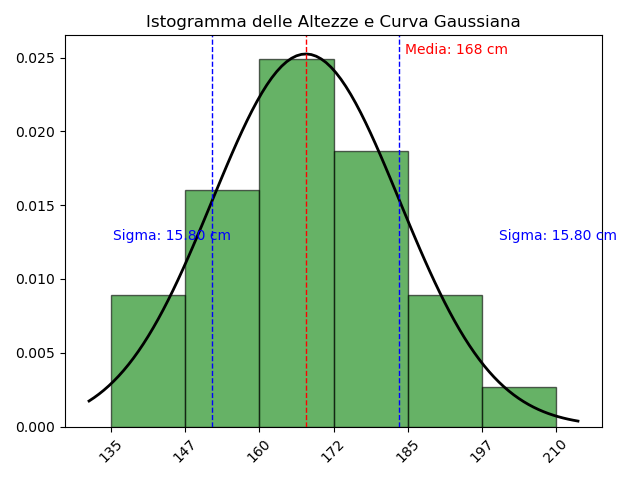
\includegraphics[width=0.8\textwidth]{istogramma.png}
    \caption{Istogramma delle Altezze con Sovrapposta la Curva Gaussiana}
    \label{fig:istogramma}
\end{figure}
Nel grafico \ref{fig:istogramma} vediamo sovrapposto l'istogramma costruito e la curva che lo approssima. L'istogramma ha in ascisse (asse X) gli intervalli di altezza e in ordinate (asse Y) un valore tale che l'area del bin sia uguale alla frazione di persone che hanno un'altezza compresa tra i suoi estremi. Ad esempio, se guardiamo l'intervallo tra 160 e 172, l'altezza è 0,025 perché $\left(172-160 \right)\times 0,025 =0,3$ ossia, il 30\% delle persone aveva un'altezza compresa tra 160 e 172 centimetri. Ancora un commento su media e deviazione standard. Notare che la curva è centrata attorno alla media (il valore $\SI{167,3}{\centi\meter}$) evidenziata dalla linea rossa tratteggiata. Notare anche le due linee blu. La distanza tra la linea verde e quella blu è proprio uguale alla deviazione standard (pari a $\SI{15,80}{\centi\meter}$ e indicata sul grafico come \textit{Sigma}), infatti $\SI{167,83}{\centi\meter} + \SI{15,80}{\centi\meter} = \SI{183,63}{\centi\meter}$ che è proprio dove si trova la linea verde. Notiamo infine che il 68\% delle misure capitano tra i valori $\SI{167,83}{\centi\meter} -\SI{15,80}{\centi\meter}$ e $\SI{167,83}{\centi\meter} +\SI{15,80}{\centi\meter}$, ossia tra $\SI{152,03}{\centi\meter}$ e $\SI{183,63}{\centi\meter}$. Questo è sempre vero. Quando abbiamo una grandezza che si distribuisce come la curva a campana (la gaussiana scoperta dallo scienziato Gauss) l'area sotto la curva, quella compresa tra le due linee blu, è sempre 0,68 ossia il 68\% delle misure che la approssimano, dovrebbero capitare tra $\overline{x} -\sigma$ e $\overline{x} + \sigma$.













\section{Cos'è il Best Fit Lineare}
In fisica, spesso siamo interessati a comprendere come due grandezze siano correlate tra loro. Un metodo comune per studiare queste relazioni è l'uso del best fit lineare, che ci permette di trovare la retta che meglio approssima i dati sperimentali. In questo documento, esploreremo cos'è il best fit lineare e come può essere utilizzato per analizzare le relazioni tra grandezze fisiche.
Il best fit lineare, o regressione lineare, è un metodo statistico utilizzato per determinare la retta che meglio approssima un insieme di dati. Questa retta minimizza la somma dei quadrati delle differenze verticali (chiamate residui) tra i punti dati osservati e i punti previsti dalla retta stessa.

\subsection{L'Equazione della Retta}
L'equazione di una retta in due dimensioni è:
\[
y = b\cdot x + a
\]
dove:
\begin{itemize}
    \item \(y\) è la variabile dipendente,
    \item \(x\) è la variabile indipendente,
    \item \(b\) è la pendenza della retta,
    \item \(a\) è l'intercetta della retta con l'asse \(y\).
\end{itemize}
Questa relazione si incontra spesso in fisica. Un esempio è il moto uniforme. In questo modo, la relazione che lega lo spazio percorso $s$, la posizione inizile $s_0$, il tempo impiegato $t$  la velocità $v$ è:
\[
s=s_0 + v\cdot t
\]
Potremmo disporre di una tabella di dati del tempo e della posizione e volere determinare la velocità e la posizione iniziale col metodo del best fit.

\subsection{Calcolo del Best Fit Lineare}
Per calcolare il best fit lineare, cioè trovare i parametri a e b e i loro errori, ci appoggeremo a delle librerie Python senza porci il problema di come vengono calcolati. Il problema è complesso e richiede di far variare i due parametri in modo cha la  distanza tra la retta e i punti sperimentali, sia la più piccola possibile, ossia la retta passi il più vicino possibile alla maggior parte dei punti sperimentali.

\section{Studio di moto rettilineo uniforme}
Il moto rettilineo uniforme (MRU) è un movimento con velocità costante. La relazione tra spazio e tempo in un moto rettilineo uniforme può essere descritta dall'equazione:
\[
s = s_0 + v \cdot t
\]
dove:
\begin{itemize}
    \item \( s \) è la posizione o spazio (che corrisponde a \( y \) nella regressione),
    \item \( s_0 \) è la posizione iniziale (che corrisponde all'intercetta \( a \)),
    \item \( v \) è la velocità costante (che corrisponde alla pendenza \( b \)),
    \item \( t \) è il tempo.
\end{itemize}
Usando la tecnica del best-fit (o regressione lineare) è possibile determinare posizione iniziale e velocità partendo da un insieme di coppie di dati (tempo, spazio). Nelle prossime sezioni vedremo nel ettaglio il procedimento.




\section{\texorpdfstring{Best Fit con \texttt{numpy} e \texttt{scipy.optimize.curve\_fit}}{Best Fit con numpy e scipy.optimize.curve_fit}}

\subsection{\texorpdfstring{\texttt{numpy} e $a + b x$}{numpy e a + b x}}

La libreria \texttt{numpy} è uno strumento potente per il calcolo scientifico in Python. Essa fornisce il supporto per array multidimensionali e una vasta gamma di funzioni matematiche. Nel contesto del best fit, \texttt{numpy} è utilizzata per manipolare i dati e applicare operazioni matematiche necessarie per il fitting.

Ad esempio, supponiamo di avere una serie di dati sperimentali che rappresentano due variabili correlate. Utilizzando \texttt{numpy}, possiamo rappresentare questi dati come array e prepararli per l'analisi. Le operazioni matematiche e la manipolazione dei dati diventano quindi più efficienti e facili da gestire.

\subsection{\texorpdfstring{\texttt{scipy} e \texttt{curve\_fit}}{scipy e curve_fit}}

La libreria \texttt{scipy} estende le funzionalità di \texttt{numpy} fornendo strumenti avanzati per l'ottimizzazione, l'integrazione, l'interpolazione, l'analisi dei segnali e molto altro. In particolare, il modulo \texttt{scipy.optimize} contiene la funzione \texttt{curve\_fit}, uno strumento molto potente per il fitting di curve.

\texttt{curve\_fit} permette di trovare i parametri di una funzione che meglio approssima i dati sperimentali. Per utilizzare \texttt{curve\_fit}, si segue un processo in due fasi principali:

\begin{enumerate}
    \item \textbf{Definire la funzione modello}: Questa è la funzione teorica che si pensa possa descrivere i dati. Può trattarsi di una retta, una parabola, una curva esponenziale o qualsiasi altra forma funzionale.
    \item \textbf{Utilizzare \texttt{curve\_fit} per trovare i parametri ottimali}: Passando la funzione modello e i dati sperimentali a \texttt{curve\_fit}, essa restituirà i parametri che meglio approssimano i dati. Questi parametri possono poi essere utilizzati per fare previsioni o per comprendere meglio la relazione tra le variabili.
\end{enumerate}

L'utilizzo congiunto di \texttt{numpy} e \texttt{scipy.optimize.curve\_fit} rende possibile affrontare in modo efficace e robusto il problema del best fit, permettendo un'analisi quantitativa precisa delle relazioni tra variabili sperimentali. Questi strumenti sono essenziali per chiunque lavori con dati numerici e desideri ottenere il massimo delle informazioni dai propri esperimenti.




\section{Misura di g}
Supponiamo di avere i seguenti dati sperimentali che descrivono la posizione di un oggetto in funzione del tempo. La posizione \( s \) è linearmente legata al tempo \( t \) con una velocità costante, ma con un piccolo errore random.

\begin{table}[h!]
\centering
\begin{tabular}{|c|c|}
\hline
Tempo (s) & Spazio (m) \\
\hline
1.0 & 2.1 \\
2.0 & 4.2 \\
3.0 & 6.1 \\
4.0 & 8.0 \\
5.0 & 10.1 \\
\hline
\end{tabular}
\caption{Tabella dei dati sperimentali per il moto rettilineo uniforme.}
\end{table}
\newpage
\section{Codice Python per la Regressione Lineare}
Il seguente codice Python esegue una regressione lineare sui dati sperimentali per determinare la velocità \( v \) e la sua incertezza.

\begin{lstlisting}[caption={Script Python per eseguire la regressione lineare}]
import numpy as np
from scipy.optimize import curve_fit
import matplotlib.pyplot as plt

# Dati sperimentali
tempo = np.array([1.0, 2.0, 3.0, 4.0, 5.0])
spazio = np.array([2.1, 4.2, 6.1, 8.0, 10.1])
error_spazio = np.array([0.1, 0.1, 0.1, 0.1, 0.1])  


# Definizione della funzione di modello lineare
def linear_model(t, s0, v):
    return s0 + v * t

# Regressione lineare
params, covariance = curve_fit(linear_model, tempo, spazio)
s0 = params[0]
v = params[1]
std_err = np.sqrt(np.diag(covariance))

# Calcolo dell'errore sulla velocità
v_error = std_err[1]

print(f"Velocità (v): {v:.2f} $\pm$ {v_error:.2f} m/s")

# Creazione del grafico
plt.figure(figsize=(8, 6))
plt.errorbar(tempo, spazio, yerr=error_spazio, fmt='o', label='Dati sperimentali', capsize=5)
plt.plot(tempo, linear_model(tempo, *params), 'r-', label='Retta di regressione')
plt.title('Moto Rettilineo Uniforme')
plt.xlabel('Tempo (s)')
plt.ylabel('Spazio (m)')
plt.legend()
plt.grid(True)
plt.savefig(   )
#se vuoi scaricare il file da google colab decommenta le righe:
#from google.colab import files
#files.download('regressione1.png')
plt.show()
\end{lstlisting}
Il risultato in output è
\begin{verbatim}
Velocità (v): 1.98 +- 0.02 m/s
\end{verbatim}
mentre il grafico è mostrato nella figura \ref{fig:vel}
 \begin{figure}[h!]
    \centering
    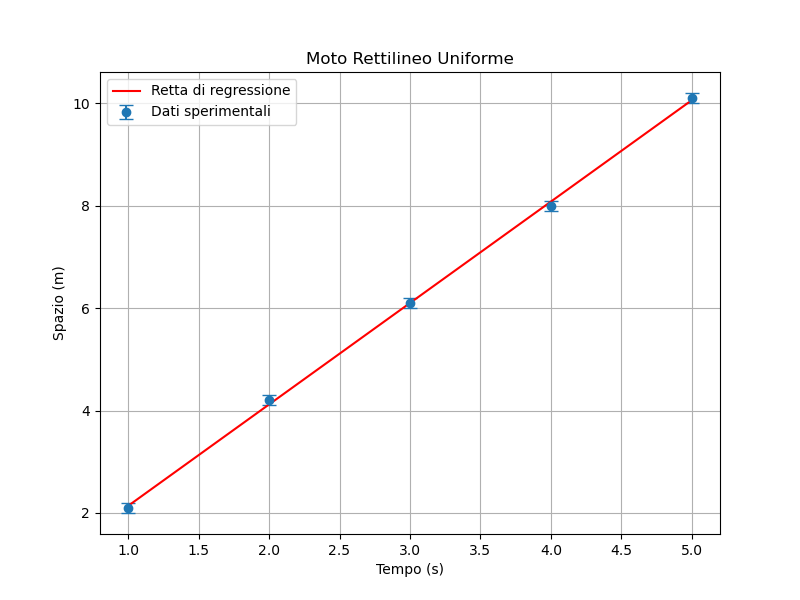
\includegraphics[scale=0.7]{velocita.png} 
    \caption{Best fit di un moto uniforme.}
    \label{fig:vel}
\end{figure}

\section{Spiegazione dei Risultati}
Il codice Python utilizza la funzione \texttt{curve\_fit} del modulo \texttt{scipy.optimize} per eseguire una regressione lineare sui dati. La funzione di modello \texttt{linear\_model} rappresenta l'equazione del moto rettilineo uniforme:
dove \( s_0 \) è l'intercetta e \( v \) è la velocità. La regressione lineare determina i valori ottimali per \( s_0 \) e \( v \) minimizzando la somma dei quadrati degli errori tra i dati osservati e i dati previsti dal modello.
Il grafico risultante mostra i dati sperimentali con le barre d'errore e la retta di regressione, che rappresenta la relazione lineare tra spazio e tempo. 
Il grafico di output è nella figura \ref{fig:vel}. Questo codice si può adattare facilmente ad altre situazioni sperimentali cambiando i dati e il nome delle grandezze (per una molla potremmo avere al posto di t ed s la lunghezza e la forza ad esempio). 




\subsection{Esempio complesso}
Supponiamo di avere i dati sperimentali nella tabella \ref{tab:regrcompl} che rappresenta i tempi di caduta di un oggetto da diverse altezze:
\begin{table}[h!]
\centering
\begin{tabular}{|c|c|}
\hline
Tempo (s) & Distanza (m) \\
\hline
1.0 & 4.9 \\
2.0 & 19.6 \\
3.0 & 44.1 \\
4.0 & 78.4 \\
5.0 & 122.5 \\
\hline
\end{tabular}
\caption{Dati di un moto di caduta.}
\label{tab:regrcompl}
\end{table}



\subsection{Analisi dei Dati}
Prima di applicare il best fit lineare, calcoliamo il tempo al quadrato \( t^2 \). Infatti la formula del moto di caduta:
\[
s=\frac{1}{2}g\cdot t^2
\]
ci dice che se pongo $t^2 =t2$, la relazione tra $s$ e  $t2$ è lineare perché la formula si scrive:
\[
s=\frac{1}{2} g \cdot t2
\]
mentre quella tra $t$ ed $s$ è quadratica. A questo punto, se poniamo  $b=\frac{g}{2}$, la relazione si può scrivere:
\[
s=b\cdot 2t
\]
essendo quindi una relazione senza parametro intercetta. Una volta trovato $b$, determiniamo l'accelerazione di gravità da una formula inversa.
\[
g = 2\cdot b
\]
e il suo errore propagato vale:
\[\sigma_g = 2\cdot \sigma_b
\]
essendo $\sigma_b$ l'errore sul parametro $b$ (nel codice, gli errori sulle $y$, sul parametro $a$ e sul parametro $b$ si ottengono dal vettorem
\begin{center}
\begin{tabular}{|c|c|}
\hline
Tempo (s) & Tempo al quadrato (s\(^2\)) \\
\hline
1.0 & 1.0 \\
2.0 & 4.0 \\
3.0 & 9.0 \\
4.0 & 16.0 \\
5.0 & 25.0 \\
\hline
\end{tabular}
\end{center}

Il codice Python per eseguire la regressione lineare e calcolare l'accelerazione di gravità è:

\begin{lstlisting}[caption={Calcolo della Regressione Lineare e Accelerazione di Gravità}]
import numpy as np
from scipy.optimize import curve_fit
import matplotlib.pyplot as plt

# Dati sperimentali
tempo = np.array([1.0, 2.0, 3.0, 4.0, 5.0])
distanza = np.array([4.9, 19.6, 44.1, 78.4, 122.5])
error_distanza = np.array([0.1, 0.1, 0.1, 0.1, 0.1])

# Calcolo di t^2
tempo_squared = tempo**2

# Definizione della funzione di modello lineare senza intercetta
def linear_model(t_squared, g_over_2):
    return g_over_2 * t_squared

# Regressione lineare forzata attraverso l'origine
params, covariance = curve_fit(linear_model, tempo_squared, distanza, sigma=error_distanza, absolute_sigma=True)
g_over_2 = params[0]

# Calcolo dell'accelerazione di gravità
g = 2 * g_over_2

# Calcolo dell'errore associato
std_err = np.sqrt(np.diag(covariance))
g_error = 2 * std_err[0]


print(f"Accelerazione di gravità (g): {g:.2f} ± {g_error:.2f} m/s^2")

# Creazione del grafico
plt.figure(figsize=(8, 6))
plt.errorbar(tempo_squared, distanza, yerr=error_distanza, fmt='o', label='Dati sperimentali', capsize=5)
plt.plot(tempo_squared, linear_model(tempo_squared, *params), 'r-', label='Retta di regressione')
plt.title('Misurazione dell\'Accelerazione di Gravità')
plt.xlabel('Tempo al quadrato (s^2)')
plt.ylabel('Distanza (m)')
plt.legend()
plt.grid(True)
plt.savefig('regressione2.png')
#se vuoi scaricare il file da google colab decommenta le righe:
#from google.colab import files
#files.download('regressione2.png')
plt.show()


\end{lstlisting}


Il grafico è mostrato in figura.\ref{fig:g}. L'output dello script è:
\begin{verbatim}
Accelerazione di gravità (g): 9.80 +- 0.01 m/s^2
\end{verbatim}

Segue spiegazione del codice.




\begin{figure}[h]
    \centering
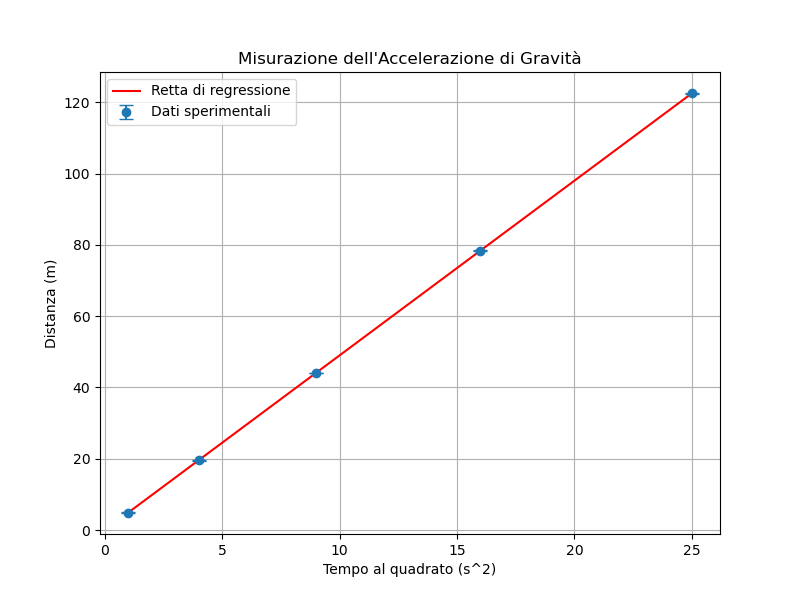
\includegraphics[scale=0.6]{g.png} 
    \caption{Grafico della regressione lineare per il calcolo dell'accelerazione dalla pendenza.}
    \label{fig:g}
\end{figure}

\section{Dettagli sul codice}

\subsection{Dati Sperimentali}
I dati di tempo e distanza sono memorizzati nei seguenti array:

\begin{itemize}
    \item \texttt{tempo}: Array contenente i valori di tempo (in secondi).
    \item \texttt{distanza}: Array contenente i valori di distanza (in metri) misurati.
    \item \texttt{error\_distanza}: Array contenente gli errori associati alle misure di distanza (in metri).
\end{itemize}

\subsection{Calcolo di \( t^2 \)}
Per adattare il modello \( d = \frac{1}{2} g t^2 \), è necessario calcolare il tempo al quadrato. Questo viene fatto con:

\begin{lstlisting}
# Calcolo del tempo al quadrato
tempo_squared = tempo**2
\end{lstlisting}

Il vettore \texttt{tempo\_squared} contiene i valori del tempo al quadrato, che sono usati per la regressione lineare.

\subsection{Definizione della Funzione di Modello}
Definiamo una funzione lineare che rappresenta la relazione tra distanza e tempo al quadrato:

\begin{lstlisting}
# Definizione della funzione lineare
def linear_model(t_squared, g_over_2):
    return g_over_2 * t_squared
\end{lstlisting}

Questa funzione modella la relazione \( d = \frac{1}{2} g t^2 \) e assume che l'intercetta sia zero. \texttt{g\_over\_2} rappresenta la metà dell'accelerazione di gravità.

\subsection{Regressione Lineare}
Utilizziamo la funzione \texttt{curve\_fit} per eseguire la regressione lineare. I parametri e la covarianza sono ottenuti da:

\begin{lstlisting}
# Regressione lineare forzata attraverso l'origine
params, covariance = curve_fit(linear_model, tempo_squared, distanza, sigma=error_distanza, absolute_sigma=True)
g_over_2 = params[0]
\end{lstlisting}

\begin{itemize}
    \item \texttt{curve\_fit}: Funzione che calcola i parametri migliori per adattare il modello ai dati.
    \item \texttt{linear\_model}: La funzione di modello lineare definita in precedenza.
    \item \texttt{tempo\_squared}: Array contenente i valori di tempo al quadrato.
    \item \texttt{distanza}: Array contenente i valori di distanza misurati.
    \item \texttt{sigma=error\_distanza}: Specifica gli errori associati alle misure di distanza.
    \item \texttt{absolute\_sigma=True}: Indica che gli errori forniti sono errori assoluti.
    \item \texttt{params}: Array contenente i parametri stimati (in questo caso, \texttt{g\_over\_2}).
    \item \texttt{covariance}: Matrice di covarianza dei parametri stimati, utilizzata per calcolare l'incertezza associata.
\end{itemize}

\subsection{Calcolo dell'Accelerazione di Gravità}
L'accelerazione di gravità \( g \) è calcolata come:

\begin{lstlisting}
# Calcolo di g
g = 2 * g_over_2
\end{lstlisting}

Poiché il nostro modello è \( d = \frac{1}{2} g t^2 \), la pendenza \( g\_over\_2 \) è la metà dell'accelerazione di gravità.

\subsection{Calcolo dell'Errore Associato}
L'errore associato a \( g \) è calcolato utilizzando la covarianza dei parametri:

\begin{lstlisting}
# Calcolo dell'errore associato
std_err = np.sqrt(np.diag(covariance))
g_error = 2 * std_err[0]

\end{lstlisting}

\begin{itemize}
    \item \texttt{np.sqrt(np.diag(covariance))}: Calcola l'errore standard dei parametri stimati.
    \item \texttt{std\_err}: Array contenente gli errori standard.
    \item \texttt{g\_error}: L'errore associato all'accelerazione di gravità \( g \), calcolato come il doppio dell'errore della pendenza \( g/2 \).
\end{itemize}

\subsection{Creazione del Grafico}
Il grafico visualizza i dati sperimentali e la retta di regressione. Le barre d'errore sono mostrate per indicare l'incertezza nella misura della distanza:

\begin{lstlisting}
# Creazione del grafico
plt.figure(figsize=(8, 6))
plt.errorbar(tempo_squared, distanza, yerr=error_distanza, fmt='o', label='Dati sperimentali', capsize=5)
plt.plot(tempo_squared, linear_model(tempo_squared, *params), 'r-', label='Retta di regressione')
plt.title('Misurazione dell\'Accelerazione di Gravità')
plt.xlabel('Tempo al quadrato (s^2)')
plt.ylabel('Distanza (m)')
plt.legend()
plt.grid(True)
plt.show()
\end{lstlisting}

\begin{itemize}
    \item \texttt{plt.figure(figsize=(8, 6))}: Crea una nuova figura di dimensioni 8x6 pollici.
    \item \texttt{plt.errorbar}: Crea un grafico a dispersione con barre d'errore per ogni punto dati.
    \item \texttt{tempo\_squared}: Array con i valori di tempo al quadrato.
    \item \texttt{distanza}: Array con i valori di distanza misurati.
    \item \texttt{yerr=error\_distanza}: Specifica gli errori associati alle misure di distanza.
    \item \texttt{fmt='o'}: Specifica che i punti dati sono rappresentati come cerchi.
    \item \texttt{label='Dati sperimentali'}: Etichetta per i dati sperimentali.
    \item \texttt{capsize=5}: Lunghezza delle barre orizzontali alle estremità delle barre d'errore.
    \item \texttt{plt.plot}: Disegna la retta di regressione.
    \item \texttt{linear\_model(tempo\_squared, *params)}: Valori previsti dal modello lineare.
    \item \texttt{'r-'}: Specifica che la retta di regressione è rossa e solida.
    \item \texttt{label='Retta di regressione'}: Etichetta per la retta di regressione.
    \item \texttt{plt.title}: Aggiunge il titolo al grafico.
    \item \texttt{plt.xlabel}: Aggiunge l'etichetta all'asse delle ascisse.
    \item \texttt{plt.ylabel}: Aggiunge l'etichetta all'asse delle ordinate.
    \item \texttt{plt.legend()}: Mostra la legenda nel grafico.
    \item \texttt{plt.grid(True)}: Aggiunge una griglia al grafico.
    \item \texttt{plt.show()}: Visualizza il grafico.
\end{itemize}




\end{document}
